% ==============================================================================
% Paper 1: RNASim (L = 1,596) Table & JC10k/JC1k (L = 10,000 / 1,000) Figure
% Uniform Random Tree Initialization + DIPPER 0.1.5 (GPU) across N = 1,000 -> 10,000,000 taxa
% ==============================================================================

\begin{table*}[tbp]
\centering
\caption{Sequence-to-tree scaling on simulated \textbf{RNASim} alignments ($L = 1{,}596$ sites) from $N = 1{,}000$ to $N = 10{,}000{,}000$ taxa. Values for $N \le 100{,}000$ report $\text{Mean} \pm \text{SD}$ across $R = 5$ independent replicates ($\text{rep} = 0..4$). All tree-refinement methods (\texttt{Phylo2Vec-Minibatch-GPU}, \texttt{VeryFastTree-ME}, \texttt{VeryFastTree-ML}, \texttt{FastTreeMP-ME}, \texttt{FastTreeMP-ML}) start from the \textbf{identical uniform random Phylo2Vec tree} ($100.0\%$ initial RF error), whereas \texttt{DIPPER 0.1.5} constructs a tree \textit{de novo} from the sequence alignment on GPU. \texttt{FastTree-ML} and \texttt{VeryFastTree-ML} are omitted for $N \ge 50{,}000$, and only \texttt{Phylo2Vec-Minibatch-GPU} scales to $N = 10{,}000{,}000$.}
\label{tab:rnasim_full_scaling}
\scriptsize
\setlength{\tabcolsep}{4.2pt}
\begin{tabular}{@{}rrlrrrrrr@{}}
\toprule
$N$ & $R$ & Method & Norm.\ RF (\%) & Time (s) & $\Delta\text{BME}$ & Host RAM (MB) & GPU VRAM (MB) & Hardware (CPU / GPU)\\
\midrule
1,000 & 5 & Uniform Random Init & $99.97 \pm 0.04$ & $0.00 \pm 0.00$ & $0.00 \pm 0.00$ & --- & --- & ---\\
1,000 & 5 & DIPPER 0.1.5 (GPU, \textit{de novo}) & $20.98 \pm 0.82$ & $0.47 \pm 0.07$ & --- & $121.6 \pm 0.5$ & $392.0 \pm 0.0$ & 64 CPU / $1\times$ A6000\\
1,000 & 5 & FastTreeMP 2.2 (\texttt{-noml -intree}) & $19.70 \pm 3.12$ & $11.94 \pm 0.20$ & --- & $133.5 \pm 2.9$ & --- & 64 CPU / 0 GPU\\
1,000 & 5 & VeryFastTree 4.0 (\texttt{-noml -intree}) & $18.62 \pm 0.89$ & $8.04 \pm 0.24$ & --- & $131.6 \pm 2.2$ & --- & 64 CPU / 0 GPU\\
1,000 & 5 & FastTreeMP 2.2 (\texttt{ME+ML -intree}) & $\mathbf{14.42 \pm 0.47}$ & $18.30 \pm 0.58$ & --- & $133.5 \pm 2.9$ & --- & 64 CPU / 0 GPU\\
1,000 & 5 & VeryFastTree 4.0 (\texttt{ME+ML -intree}) & $14.62 \pm 0.65$ & $9.42 \pm 0.27$ & --- & $133.5 \pm 2.9$ & --- & 64 CPU / 0 GPU\\
1,000 & 5 & \textbf{Phylo2Vec-Minibatch-GPU} & $18.31 \pm 1.19$ & $\mathbf{0.04 \pm 0.00}$ & $\mathbf{-144.10 \pm 1.45}$ & $735.7 \pm 1.4$ & $690.8 \pm 0.0$ & 64 CPU / $1\times$ H100\\
\midrule
5,000 & 5 & Uniform Random Init & $100.00 \pm 0.00$ & $0.00 \pm 0.00$ & $0.00 \pm 0.00$ & --- & --- & ---\\
5,000 & 5 & DIPPER 0.1.5 (GPU, \textit{de novo}) & $18.82 \pm 0.77$ & $2.07 \pm 0.06$ & --- & $133.0 \pm 0.0$ & $580.0 \pm 0.0$ & 64 CPU / $1\times$ A6000\\
5,000 & 5 & FastTreeMP 2.2 (\texttt{-noml -intree}) & $45.55 \pm 9.45$ & $70.38 \pm 1.91$ & --- & $290.4 \pm 0.5$ & --- & 64 CPU / 0 GPU\\
5,000 & 5 & VeryFastTree 4.0 (\texttt{-noml -intree}) & $43.17 \pm 9.67$ & $42.96 \pm 0.86$ & --- & $317.6 \pm 7.4$ & --- & 64 CPU / 0 GPU\\
5,000 & 5 & FastTreeMP 2.2 (\texttt{ME+ML -intree}) & $\mathbf{13.62 \pm 1.33}$ & $117.48 \pm 5.45$ & --- & $292.2 \pm 1.8$ & --- & 64 CPU / 0 GPU\\
5,000 & 5 & VeryFastTree 4.0 (\texttt{ME+ML -intree}) & $14.85 \pm 1.41$ & $50.22 \pm 1.55$ & --- & $318.6 \pm 8.0$ & --- & 64 CPU / 0 GPU\\
5,000 & 5 & \textbf{Phylo2Vec-Minibatch-GPU} & $14.80 \pm 0.62$ & $\mathbf{0.49 \pm 0.05}$ & $\mathbf{-869.75 \pm 6.89}$ & $739.9 \pm 0.7$ & $696.8 \pm 0.0$ & 64 CPU / $8\times$ H100\\
\midrule
10,000 & 5 & Uniform Random Init & $100.00 \pm 0.00$ & $0.01 \pm 0.01$ & $0.00 \pm 0.00$ & --- & --- & ---\\
10,000 & 5 & DIPPER 0.1.5 (GPU, \textit{de novo}) & $17.78 \pm 0.38$ & $8.90 \pm 0.10$ & --- & $145.8 \pm 0.8$ & $1156.0 \pm 0.0$ & 64 CPU / $1\times$ A6000\\
10,000 & 5 & FastTreeMP 2.2 (\texttt{-noml -intree}) & $64.34 \pm 7.47$ & $155.42 \pm 5.57$ & --- & $570.1 \pm 1.3$ & --- & 64 CPU / 0 GPU\\
10,000 & 5 & VeryFastTree 4.0 (\texttt{-noml -intree}) & $58.97 \pm 6.78$ & $90.56 \pm 3.09$ & --- & $542.3 \pm 7.1$ & --- & 64 CPU / 0 GPU\\
10,000 & 5 & FastTreeMP 2.2 (\texttt{ME+ML -intree}) & $14.47 \pm 1.33$ & $280.93 \pm 11.76$ & --- & $571.8 \pm 1.3$ & --- & 64 CPU / 0 GPU\\
10,000 & 5 & VeryFastTree 4.0 (\texttt{ME+ML -intree}) & $14.29 \pm 0.59$ & $103.90 \pm 3.22$ & --- & $545.0 \pm 6.8$ & --- & 64 CPU / 0 GPU\\
10,000 & 5 & \textbf{Phylo2Vec-Minibatch-GPU} & $\mathbf{13.65 \pm 0.40}$ & $\mathbf{1.39 \pm 0.66}$ & $\mathbf{-1868.34 \pm 9.98}$ & $743.8 \pm 1.1$ & $700.8 \pm 0.0$ & 64 CPU / $8\times$ H100\\
\midrule
50,000 & 5 & Uniform Random Init & $100.00 \pm 0.00$ & $0.04 \pm 0.00$ & $0.00 \pm 0.00$ & --- & --- & ---\\
50,000 & 5 & DIPPER 0.1.5 (GPU, \textit{de novo}) & $19.50 \pm 0.15$ & $59.83 \pm 5.51$ & --- & $246.6 \pm 0.8$ & $446.0 \pm 0.0$ & 64 CPU / $1\times$ A6000\\
50,000 & 5 & FastTreeMP 2.2 (\texttt{-noml -intree}) & $89.30 \pm 1.13$ & $874.43 \pm 24.09$ & --- & $2835.9 \pm 0.6$ & --- & 64 CPU / 0 GPU\\
50,000 & 5 & VeryFastTree 4.0 (\texttt{-noml -intree}) & $88.09 \pm 1.29$ & $486.95 \pm 38.28$ & --- & $2405.4 \pm 15.5$ & --- & 64 CPU / 0 GPU\\
50,000 & 5 & \textbf{Phylo2Vec-Minibatch-GPU} & $\mathbf{9.91 \pm 0.15}$ & $\mathbf{3.71 \pm 0.19}$ & $\mathbf{-10943.39 \pm 12.09}$ & $782.2 \pm 1.1$ & $746.8 \pm 0.0$ & 64 CPU / $8\times$ H100\\
\midrule
100,000 & 5 & Uniform Random Init & $100.00 \pm 0.00$ & $0.10 \pm 0.00$ & $0.00 \pm 0.00$ & --- & --- & ---\\
100,000 & 5 & DIPPER 0.1.5 (GPU, \textit{de novo}) & $16.80 \pm 0.19$ & $216.26 \pm 0.22$ & --- & $386.5 \pm 2.8$ & $512.0 \pm 0.0$ & 64 CPU / $1\times$ A6000\\
100,000 & 5 & FastTreeMP 2.2 (\texttt{-noml -intree}) & $92.62 \pm 0.59$ & $1853.11 \pm 67.03$ & --- & $5677.2 \pm 2.3$ & --- & 64 CPU / 0 GPU\\
100,000 & 5 & VeryFastTree 4.0 (\texttt{-noml -intree}) & $92.73 \pm 1.37$ & $1024.52 \pm 37.34$ & --- & $4651.7 \pm 24.7$ & --- & 64 CPU / 0 GPU\\
100,000 & 5 & \textbf{Phylo2Vec-Minibatch-GPU} & $\mathbf{8.76 \pm 0.05}$ & $\mathbf{6.75 \pm 0.30}$ & $\mathbf{-23262.65 \pm 20.42}$ & $830.2 \pm 0.9$ & $794.8 \pm 0.0$ & 64 CPU / $8\times$ H100\\
\midrule
1,000,000 & 1 & Uniform Random Init & $100.00$ & $0.00$ & $0.00$ & --- & --- & ---\\
1,000,000 & 1 & DIPPER 0.1.5 (GPU, \textit{de novo}) & $11.25$ & $978.23$ & --- & $4189.6$ & $1871.8$ & 64 CPU / $1\times$ A6000\\
1,000,000 & 1 & \textbf{Phylo2Vec-Minibatch-GPU} & $\mathbf{1.17}$ & $\mathbf{69.01}$ & $\mathbf{-306164.97}$ & $\mathbf{1043.5}$ & $\mathbf{1656.8}$ & 64 CPU / $8\times$ H100\\
\midrule
10,000,000 & 1 & Uniform Random Init & $100.00$ & $0.00$ & $0.00$ & --- & --- & ---\\
10,000,000 & 1 & \textbf{Phylo2Vec-Minibatch-GPU} & $\mathbf{4.13}$ & $\mathbf{974.61}$ & $\mathbf{-3319791.02}$ & $\mathbf{2575.1}$ & $10240.8$ & 64 CPU / $8\times$ H100\\
\bottomrule
\end{tabular}
\end{table*}

\begin{figure*}[tbp]
\centering
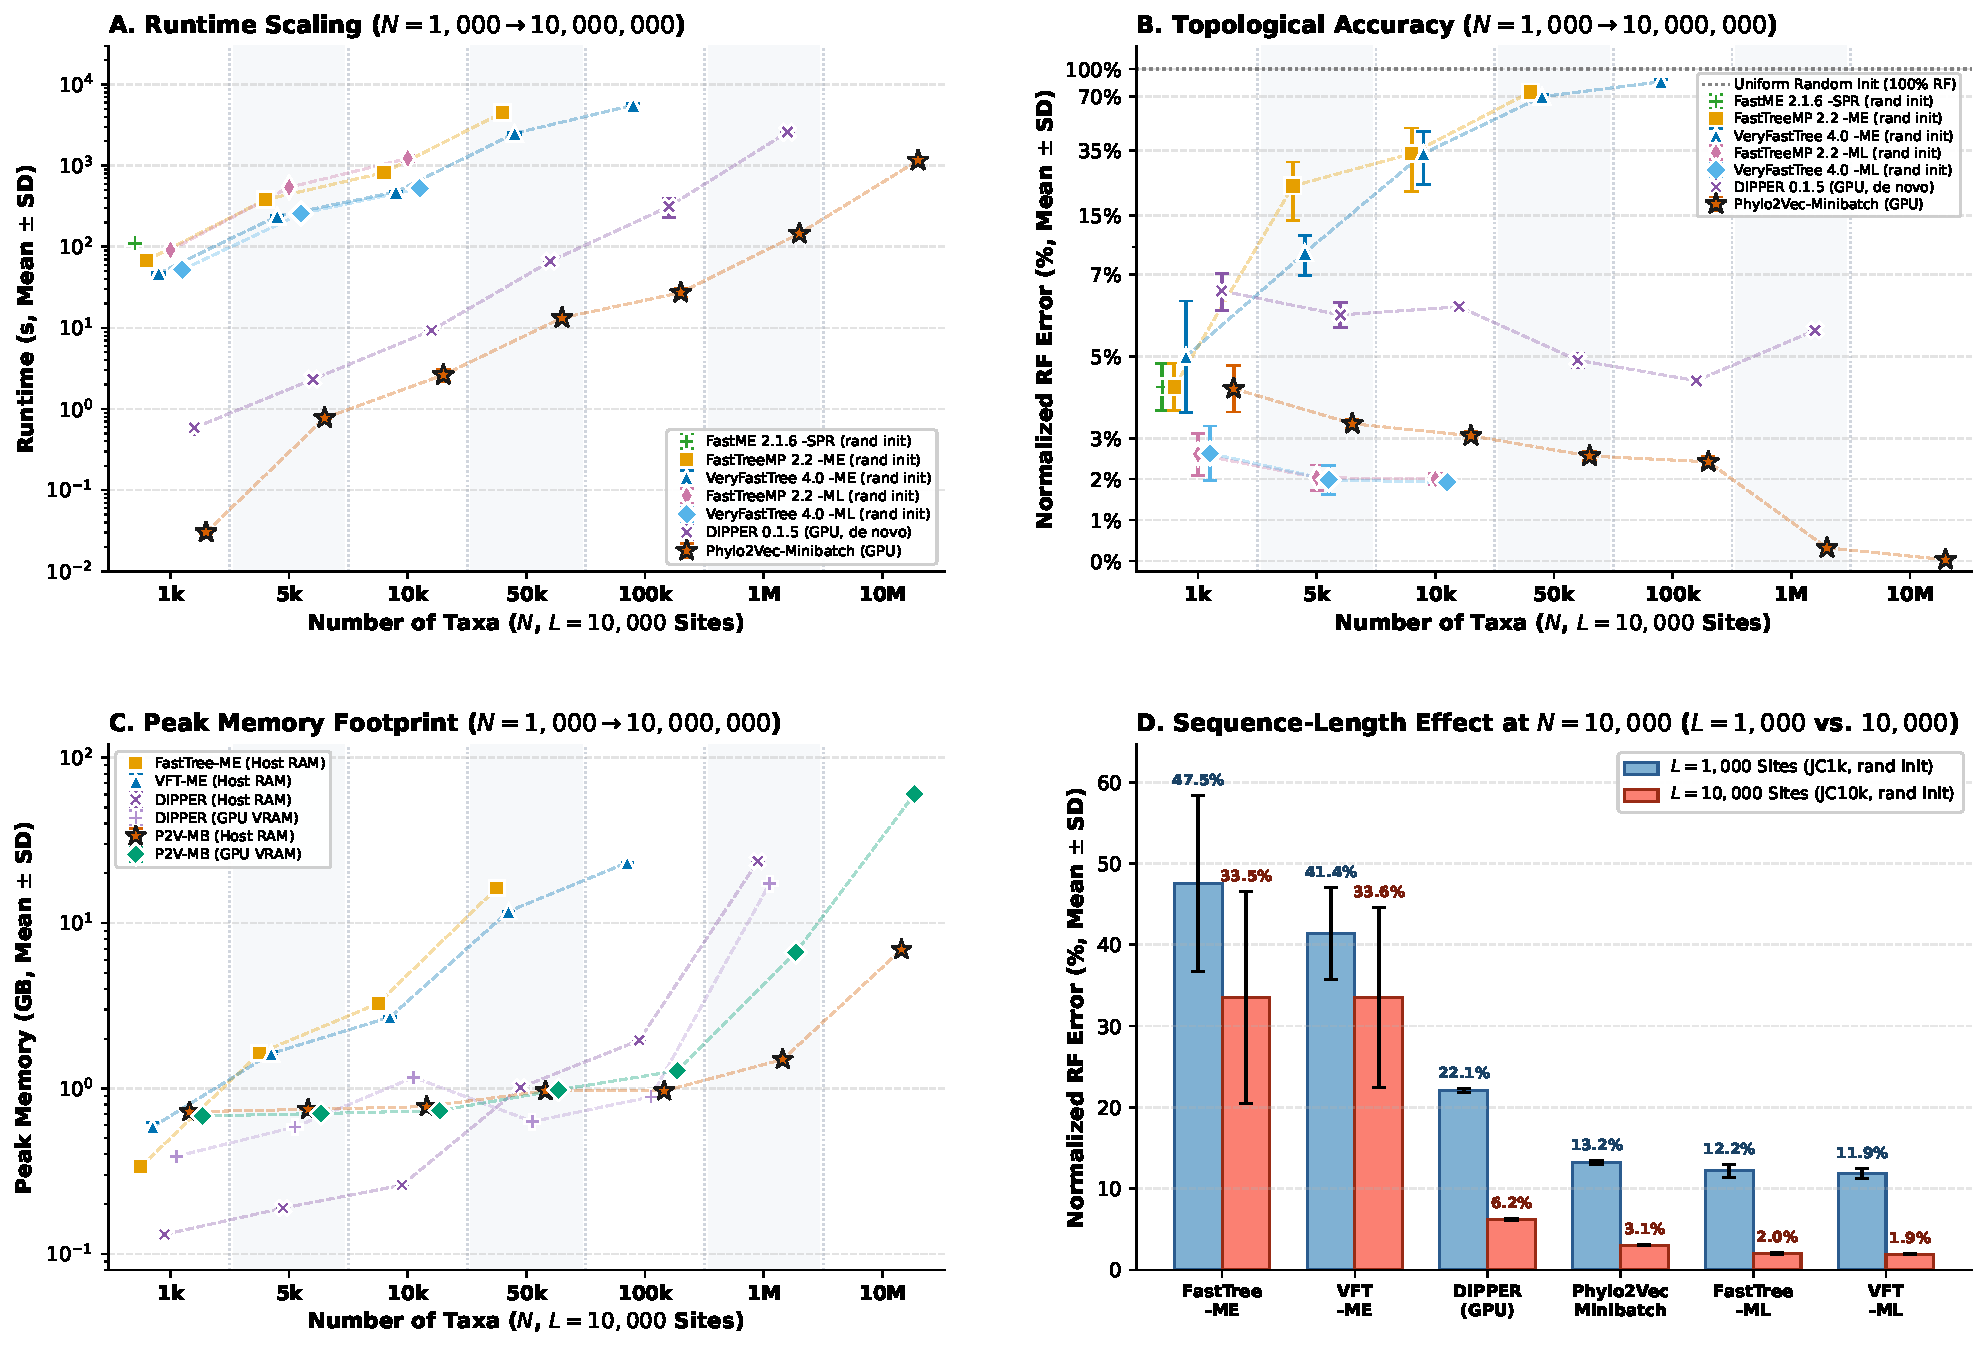
\includegraphics[width=\textwidth]{figures/paper1_jc_scaling_figure.pdf}
\caption{Sequence-to-tree scaling on simulated Jukes--Cantor alignments across $N = 1{,}000$ to $N = 10{,}000{,}000$ taxa starting from uniform random trees ($R = 5$ independent replicates for $N \le 100{,}000$; $\text{Mean} \pm 1\text{ SD}$ error bars and shaded bands), alongside \texttt{DIPPER 0.1.5 (GPU)}. \textbf{(A)} Runtime scaling on $L = 10{,}000$ sites (\texttt{JC10k}). \textbf{(B)} Topological error (normalized Robinson--Foulds percentage) on $L = 10{,}000$ sites (\texttt{JC10k}). \textbf{(C)} Peak Host RAM and GPU VRAM footprint across $N = 1{,}000 \to 10{,}000{,}000$. \textbf{(D)} Effect of sequence length ($L = 1{,}000$ vs.\ $L = 10{,}000$ sites) on topological accuracy at $N = 10{,}000$ taxa.}
\label{fig:jc_scaling_4panel}
\end{figure*}
